\documentclass[12pt, a4paper]{article}

\usepackage[utf8]{inputenc}
\usepackage[T1]{fontenc}
\usepackage[francais]{babel}
\usepackage[top=2cm, bottom=2cm, left=2cm, right=2cm]{geometry}
\usepackage{verbatim}
\usepackage{graphicx}
\usepackage{listings}
\usepackage[dvipsnames]{xcolor}
\lstset{
%upquote=true,
columns=flexible,
basicstyle=\ttfamily,}

\title{Projet IHM -- RICM4}
\author{\bsc{Fréby} Rodolphe -- \bsc{Barbier} Jérome -- \bsc{Husson} Augustin -- \bsc{Labat} Paul}
\date{\today}



\begin{document}
\maketitle
\tableofcontents
\newpage

\textcolor{Violet}{\section{Introduction}}
L'objectif de ce rapport est de présenter le logiciel ConcurTaskTree Environnement (CTTE), en étudiant et analysant son ergonomie. Il s'agit d'un outil pour la création et la modification, via une interface graphique, d'un arbre de tâches, qui n'est pas dans sa version actuelle fait pour des novices. Notre groupe a donc pour objectif d'étudier le logiciel, de proposer une solution alternative, et enfin de la réaliser. Tout au long de ce premier rapport, nous allons fournir une analyse critique de CTTE, de mettre en évidence ses forces et ses faiblesses en nous appuyant sur les critères ergonomiques de Scapin et Bastien.  

\textcolor{Violet}{\section{Guidage}}
Cette première partie regroupe 4 sous-critères, l'incitation, le groupement / distinction entre items, le feedback immédiat et la lisibilité. Le guidage représente l'ensemble des moyens qui sont mis en œuvre pour informer, conseiller et diriger au mieux l'utilisateur lors de ses interactions avec l'ordinateur. 

\textcolor{NavyBlue}{\subsection{Incitation}}
Cette première sous partie recouvre les moyens mis en place afin d'expliciter à un utilisateur les actions qu'il peut effectuer. Cela permet à l'utilisateur de savoir dans quel contexte il se trouve.\\

Dans le cadre de CTTE, le logiciel nous indique bien quel bouton nous avons sélectionné grâce à un verrouillage sur l'image de celui-ci. 


\begin{figure}[h]
\begin{center}
   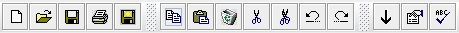
\includegraphics{incitation.jpg}
	\caption{On remarque bien quel bouton est sélectionné}
	\end{center}
\end{figure}


Cependant, nous remarquons que les actions n'étant pas réalisables ne voient pas leur bouton grisé, bloqué, ce qui n'aide pas l'utilisateur à repérer les actions autorisées dans le contexte dans lequel l'utilisateur se situe.
\newpage
\textcolor{NavyBlue}{\subsection{Groupement / Distinction entre items}}
Ce critère concerne l'organisation des différentes fonctionnalités les unes par rapport aux autres, de leur regroupement entre elles ou non.\\


On remarque dans CTTE que dans l'ensemble, les groupes de fonctionnalités sont généralement bien séparés, avec un trait marquant bien les limites. Comme vous pouvez le remarquer avec l'image ci-dessous, les éléments liés aux modifications générales du document sont regroupés en haut à gauche (1), ceux pour la gestion des opérateurs sur les arbres sont regroupés sur la gauche de la zone de travail (2), et ainsi de suite pour la totalité des blocs. 


\begin{figure}[h]
\begin{center}
   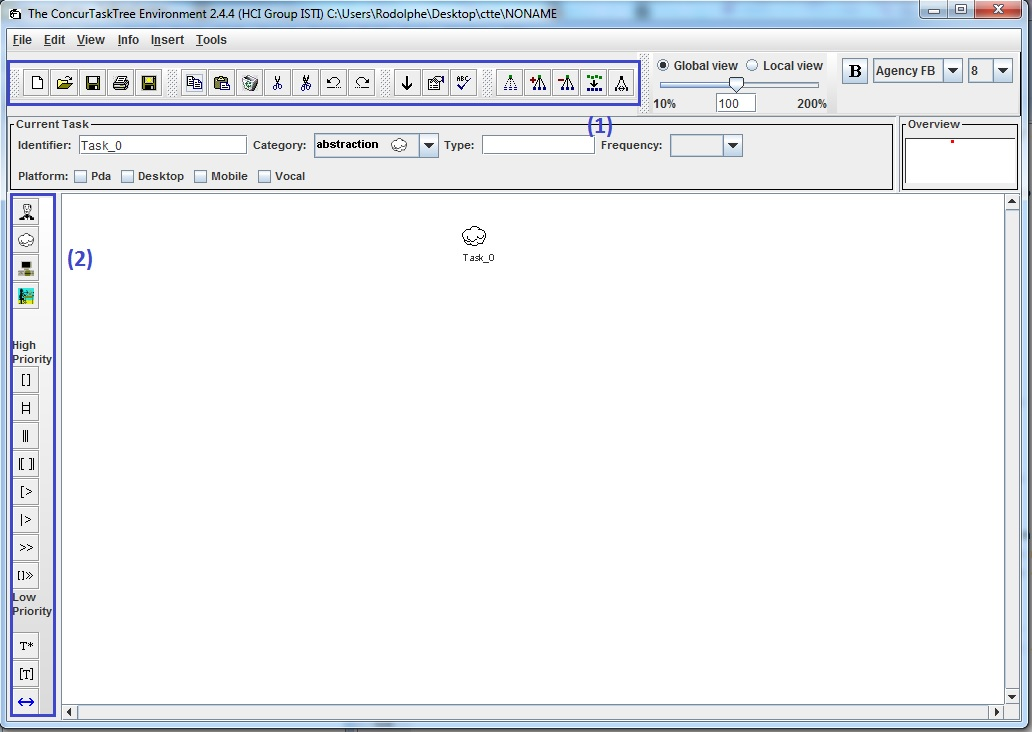
\includegraphics[scale = 0.5]{groupement.jpg}
	\caption{Les fonctions sont regroupées par ensemble}
	\end{center}
\end{figure}
Il en est de même pour les différents menus déroulants, regroupant des groupes de fonctionnalités ensemble, et les séparant en de sous groupe de manière distincte.
\begin{figure}[h]
\begin{center}
   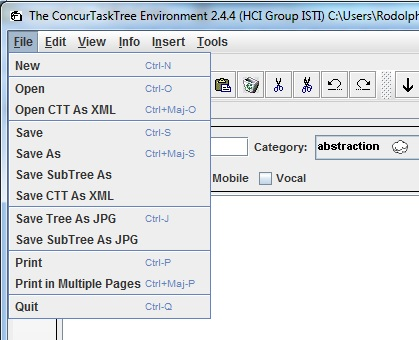
\includegraphics[scale = 0.5]{menusderoulant.jpg}
	\caption{Le regroupement des options dans le menu \emph{File}}
	\end{center}
\end{figure}

\newpage
Par contre, nous pouvons noter un léger souci quant au déplacement de certains blocs, sur le premier bandeau horizontal. Nous ne pouvons les placers comme nous le souhaitons. Le bloc déplacé se retrouve forcément au fond à droite, ou hors du logiciel. On peut aussi remarquer que les boutons liés à la police de caractère ne sont pas forcément bien placés.\\ 

\begin{figure}[h]
\begin{center}
   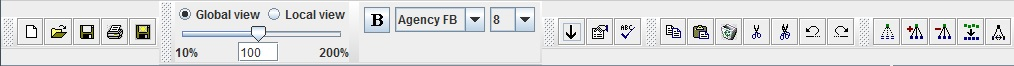
\includegraphics[scale = 0.5]{agencement.jpg}
	\caption{Les différents groupes de boutons ne sont positionnés que par décalage à droite}
	\end{center}
\end{figure}


Néanmoins, dans son ensemble, le logiciel possède une architecture des différentes fonctionnalités qui nous parait cohérente.  

\textcolor{NavyBlue}{\subsection{Feedback immédiat}}
Cette partie permet de montrer à l'utilisateur que les actions qu'il a effectuées ont bien été prises en compte par le système.\\


Notre première remarque se porte sur la sauvegarde du document. En effet, au moment d'effectuer celle-ci, aucun message ou indication n'est envoyé à l'utilisateur (le bouton sauvegarder n'est pas grisé) pour lui confirmer que son document a bien été enregistré. De même, le zoom n'est pas en temps réel, ne permettant pas à l'utilisateur de voir directement les modifications qu'il effectue. 


Cependant, pour la création d'arbres par exemple on remarque bien que la demande a été prise en compte, puisque celui-ci se construit à chaque clic. De plus, en passant simplement sa souris sur un bouton, l'utilisateur peut observer une modification de la couleur du fond, lui indiquant bien quel bouton il survole avec sa souris, en plus d'avoir un message donnant le nom de celui-ci.
\newpage
\textcolor{NavyBlue}{\subsection{Lisibilité}}
Le dernier point est la lisibilité. Cela correspond à l'idée que les informations données à l’utilisateur soient facilement compréhensibles et cohérentes pour lui, et qu'elles soient facilement visibles.


Un premier problème se pose dans le logiciel CTTE par rapport au fait que l'interface est bien trop chargée de bouton. Un utilisateur novice aura rapidement du mal à s'y retrouver, se perdant dans la masse de fonctionnalités présentées par les différents boutons, souvent bien trop petits. Nous remarquons également que certains boutons représentent des actions très spécifiques, qu'un nouvel utilisateur n'arrivera pas à comprendre sans une aide extérieure.\\ 
La police de caractère des différents nœuds et feuilles de l'arbre n'est également pas assez grande pour être lue correctement, et n'est pas forcément une police de caractère agréable (\emph{Agency FB}), et l'ajout continuel de branches entre les différents nœuds et feuilles se fait sur les noms des tâches, rendant difficile la lecture. Un dernier problème provient du fait qu'après une copie, on se retrouve avec des noms en doubles, donc il peut être difficile en récupérant le document quelques jours après une session de travail de se souvenir de qu'elle tâche était la tâche originelle si le nom n'avait pas été changé. 
\begin{figure}[h]
\begin{center}
   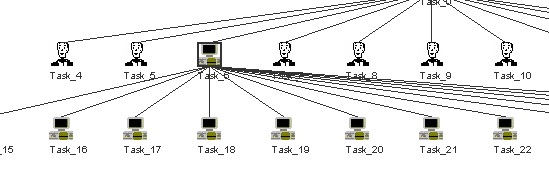
\includegraphics[scale = 0.7]{empilement.jpg}
	\caption{Il devient difficile de lire le nom de certaines tâches...}
	\end{center}
\end{figure}

\begin{figure}[h]
\begin{center}
   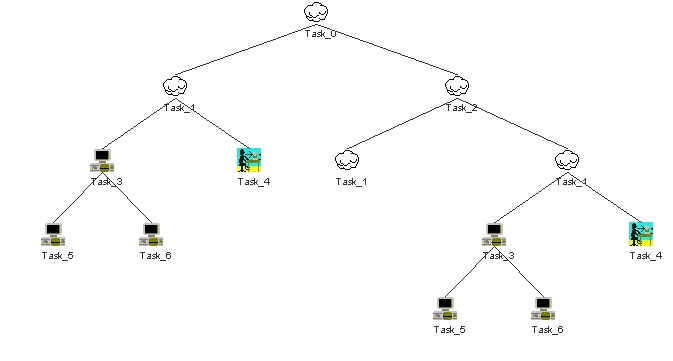
\includegraphics[scale = 0.7]{copierate.jpg}
	\caption{Après une copie, on remarque bien que certaines tâches ont le même nom}
	\end{center}
\end{figure}
\newpage
\textcolor{Violet}{\section{Charge de travail}}
Ce critère évalue la facilité de l'utilisateur à atteindre ses objectifs, de la manière la plus rapide et la plus facile possible. Celui-ci est divisé en 2 sous-critères : la brièveté et la densité informationnelle.

\textcolor{NavyBlue}{\subsection{Brièveté}}
Dans un logiciel, les éléments de l'interface ne doivent pas donner un nombre trop important d'informations diverses à un utilisateur, pour éviter celui-ci à tout mémoriser.\\


Pour le logiciel CTTE, on remarque qu'une fois le logiciel prit en main, la création d'un arbre se fait simplement, sans avoir à passer par un grand nombre d'étapes. C'est en général le cas pour la grande partie des actions. 


De plus, la plupart des éléments de l'interface en eux-mêmes ne demandent pas nécessairement un effort conséquent de mémorisation, notamment par le fait qu'ils ne contiennent pas un nombre énorme d'informations.

\textcolor{NavyBlue}{\subsection{Densité informationnelle}}
La limitation de la charge de travail passe également par la pertinence des contenues livrée à l'utilisateur. Il faut limiter au mieux le nombre d'informations présentées en même temps.\\


Comme expliqué précédemment, CTTE est bien trop chargé. Par exemple, les options de modifications de la police peuvent ne pas être affichées, mais disponibles dans les propriétés d'un nœud / feuille, la possibilité d'enregistrer en \emph{JPG}, la possibilité d'imprimer, ou d'ouvrir un nouveau document. Nous avons remarqué pendant l'utilisation du logiciel que ces fonctionnalités n'étaient pas utilisées souvent, et donc d'une certaine manière surchargent l'interface. L'icône corbeille n'est pas forcément utile également en elle même, la suppression étant généralement effectuée par la pression sur la touche \emph{Suppr}. \\


Ce genre d'option peut en règle générale être simplement laissé dans les différents menus déroulants aux endroits adéquats.

\textcolor{Violet}{\section{Contrôle explicite}}
Le contrôle explicite exprime la prise en compte par le système des actions des utilisateurs et le contrôle de ceux-ci sur le traitement de leur section. Deux sous-critères participent à cela : action explicite et contrôle utilisateur.
\textcolor{NavyBlue}{\subsection{Actions explicites}}
Ce critère concerne la relation entre le fonctionnement de l'application et les actions des utilisateurs. L'ordinateur doit exécuter seulement les actions demandées par l'utilisateur.\\


Lors de l'utilisation du logiciel, nous avons pu remarquer qu'aucune action n'était effectuée sans demande de l'utilisateur, par elle-même. L'utilisateur possède bien le contrôle du système. Néanmoins, on remarque la perte de contrôle d'un noeud / d'une feuille lors d'un \emph{drag and drop} si on déplace la souris trop rapidement.

\textcolor{NavyBlue}{\subsection{Contrôle utilisateur}}
L'utilisateur doit toujours avoir la main, et pouvoir contrôler le déroulement des traitements informatiques en cours. \\


Tout d'abord, le logiciel permet d'effectuer une action arrière aussi longtemps que cela est possible, permettant à l'utilisateur d'annuler une modification qu'il aurait effectuée après le début, celle-ci étant conservée depuis le début de la session. Il peut également s'il le souhaite revenir en avant (avec un petit souci de raccourcis clavier \emph{CNTRL + Z} doublement affecté pour le retour arrière/avant).

\begin{figure}[h]
\begin{center}
   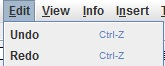
\includegraphics[scale = 0.8]{ctrlz.jpg}
	\caption{Un raccourci clavier est affecté deux fois}
	\end{center}
\end{figure}

Pour ce qui est de la possibilité de l'annulation d'un traitement en cours, nous n'avons pas réussi à trouver la possibilité de le faire, car nous n'avons pas vu d'action prenant un temps suffisamment considérable pour avoir la possibilité de l'annuler.

\textcolor{Violet}{\section{Adaptabilité}}
Ce critère concerne la capacité d'un système à réagir selon le contexte, et également selon les préférences et besoins de l'utilisateur. Deux sous-critères sont à démarquer : flexibilité et prise en compte de l'expérience utilisateur. 

\textcolor{NavyBlue}{\subsection{Flexibilité}}
Pour cette section, nous avons cherché à vérifier si l'utilisateur pouvait personnaliser l'interface afin de prendre en compte ses habitudes de travail. \\


Certaines barres d'outils sont déplaçables, mais comme exprimées précédemment, elles sont certes extractibles, mais difficilement déplaçables à la convenance de l'utilisateur. De plus, les boutons sont associés à leur barre, qui n'est pas en elle-même personnalisable. Il aurait été intéressant de permettre à l'utilisateur d'ajouter ou d'enlever des boutons en fonction de ses habitudes de travail.
\begin{figure}[h]
\begin{center}
   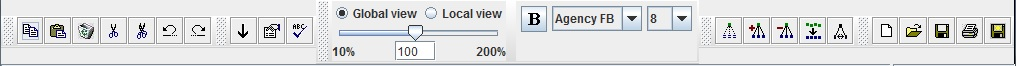
\includegraphics[scale = 0.5]{bazzare.jpg}
	\caption{On remarque vite que le placement devient bizarre et mal organisé}
	\end{center}
\end{figure}
\newpage
\textcolor{NavyBlue}{\subsection{Prise en compte de l'expérience utilisateur}}
Nous allons maintenant analyser les différents moyens misent en oeuvre afin de prendre en compte le niveau d'expérience de l'utilisateur.\\


En premier lieu, le logiciel ne fournit que très peu d'aide pour un utilisateur débutant. L'interface est la même que l'utilisateur débute où soit un expert. Un novice n'est pas guidé afin de pouvoir facilement apprendre les différentes fonctionnalités. De plus, l'indication quand un utilisateur passe sa souris sur un bouton ne fait que donner le nom de celui-ci, ne l'aidant pas à comprendre forcément son utilisation.
\begin{figure}[h]
\begin{center}
   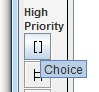
\includegraphics[scale = 1]{imagebtn.jpg}
	\caption{Le mot \emph{Choice} seul n'aide pas à la compréhension}
	\end{center}
\end{figure}

En revanche, on notera la présence de raccourcis clavier, qui sont un plus pour les utilisateurs confirmés, même si comme expliqué précédemment le raccourci \emph{CNTRL + Z} est affecté à deux actions distinctes.
%affichage du double cntrl + z

\textcolor{Violet}{\section{Gestion des erreurs}}
La gestion des erreurs concerne tous les moyens qui permettent d'éviter ou bien de réduire les erreurs, mais également de les corriger si celles-ci surviennent.

\textcolor{NavyBlue}{\subsection{Protection contre les erreurs}}
Nous allons dans un premier temps chercher les moyens mis en œuvre pour détecter et prévenir les erreurs faites par l'utilisateur. \\


Nous remarquons d'abord qu'il n'est pas possible de sélectionner deux boutons en même temps, ce qui en est une bonne chose. Cependant, les boutons qui ne devraient pas pouvoir être utilisés ne sont pas grisés. Un autre point est également à noter : lorsqu'un utilisateur modifie le champ type dans \emph{current task}, il peut rentrer n'importe quelle valeur, alors qu'il semblerait qu'une valeur spécifique soit attendue (visible en cherchant en particulier les propriétés du noeud / de la feuille). On ne sait pas si la modification est ou non prise en compte par le système, si celui-ci à traiter l'erreur, ce qui est déroutant pour l'utilisateur.
\newpage
\textcolor{NavyBlue}{\subsection{Qualité des messages d'erreur}}
L'importance d'un message d'erreur est d'être pertinent et de faciliter la lecture de l'information donnée à l'utilisateur quant à la nature de l'erreur commise.\\


Pour cela, lors de l'apparition d'une fenêtre signalant une erreur (notamment lorsqu'on clic sur \emph{check model structure}, nous remarquons un message d'erreur clair nous indiquant la localisation de l'erreur avec la possibilité de mettre en surbrillance celle-ci. Nous avons également l'information de pourquoi l'erreur s'est produite. %image d'une erreur

\begin{figure}[h]
\begin{center}
   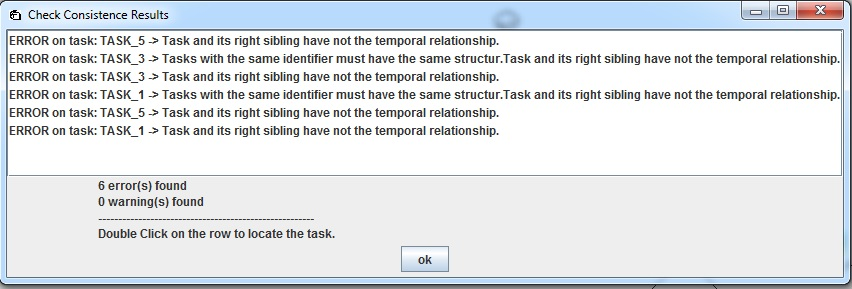
\includegraphics[scale = 0.7]{erreur.jpg}
	\caption{L'erreur est bien explicitée}
	\end{center}
\end{figure}

\textcolor{NavyBlue}{\subsection{Correction des erreurs}}
Enfin, nous allons analyser les moyens mis à la disposition de l'utilisateur pour lui permettre de corriger ses erreurs.\\


Dans un premier lieu, nous avons vu que des erreurs n'étaient pas signalées. Il est difficile dans ce cas d'avoir une correction de celles-ci. Dans l'autre cas, il n'y a pas de correction automatique, mais la clarté du message permet à l'utilisateur de corriger un problème de manière assez simple, manuellement.
\textcolor{Violet}{\section{Homogénéité et cohérence}}
Ce critère vérifie si les choix qui ont été faits auraient été respectés.\\


On remarque d'abord que les opérations sur les nœuds / feuilles fonctionnent de la même façon, ce qui respecte le principe d'homogénéité. Il en est de même avec la création des tâches, qui fonctionnent toutes selon le même principe.
\newpage
\textcolor{Violet}{\section{Signifiance des codes et dénomination}}
Cette section a pour but d'évaluer si les informations fournies par l'interface sont suffisamment explicites.

Pour CTTE, on remarque que les boutons ont un message associé, qui avec l'image, permet de déterminer pour la plupart d'entre eux leur utilisation, celle-ci étant connue par ``habitude'' : sauvegarder, imprimer, nouveau fichier... De plus, les différents onglets renferment les options telles qu'elles le sont dans la plupart des applications. Ainsi on retrouve dans \emph{File} : nouveau, sauvegarder, imprimer. Dans \emph{Edit} : copier, coller, retour arrière. Cependant, un novice ne comprendra pas nécessairement l'ensemble des termes, ce qui est ennuyeux, par exemple pour \emph{Fold / Unfold SubTree}.

\textcolor{Violet}{\section{Compatibilité}}
Nous allons maintenant analyser la réponse de CTTE par rapport à l'environnement de l'utilisateur, et si celui-ci s'adapte.


Pour l'utilisation sous Windows, on ne remarque rien de dérangeant, que le système d'exploitation soit XP, Vista, Seven ou Eight. Pour Debian, et Ubuntu avec Gnome, aucun détail ne semble ressortir, par contre, pour Mac OS, on remarque un souci quant à l'affichage, qui ne respecte pas l'homogénéité des applications. En effet, la barre de menu est normalement associée à la barre des tâches du système, comme vous pouvez le voir ci-dessous.

\begin{figure}[h]
   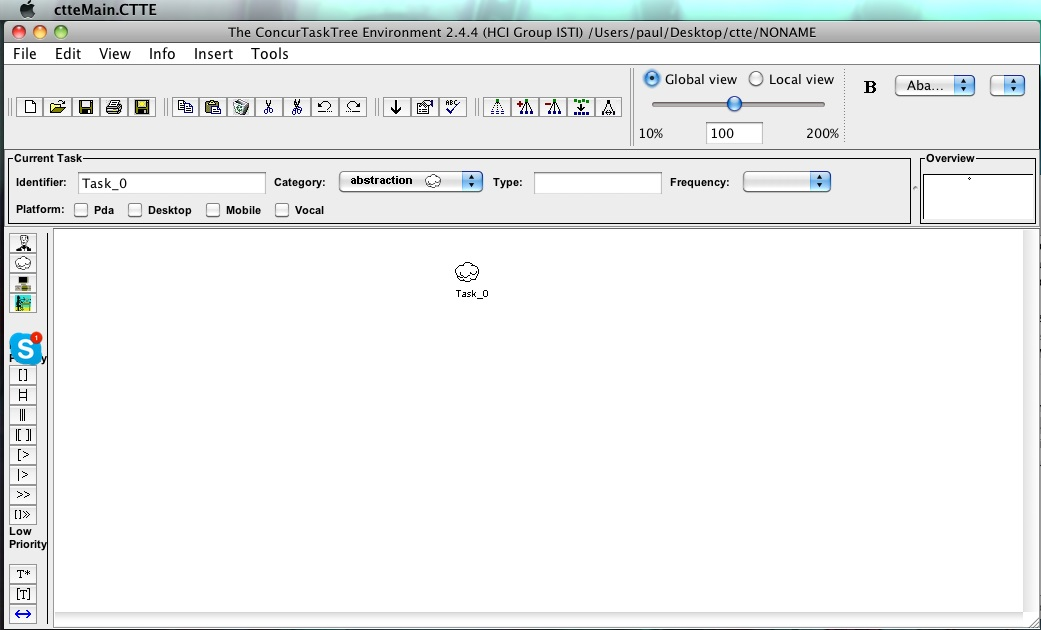
\includegraphics[scale = 0.5]{SoucisIHM.jpg}
	\caption{CTTE sous MAC, on remarque un souci au niveau de l'affichage de la barre des menus}
\end{figure}

\textcolor{Violet}{\section{Conclusion}}
Globalement, on peut dire que l'interface est fonctionnelle, mais n'est pas particulièrement facile à prendre en main à moins de faire 
des tests poussés pour en connaître toutes les fonctionnalités. Nous allons donc tâcher de perfectionner cette interface. 
Nous nous concentrerons uniquement sur son amélioration. C'est pourquoi le noyau fonctionnel ne sera pas (ré)implémenté.
\end{document}